\documentclass[letterpaper,11pt]{article}

\usepackage{latexsym}
\usepackage[empty]{fullpage}
\usepackage{titlesec}
\usepackage{marvosym}
\usepackage[usenames,dvipsnames,svgnames,table]{xcolor}
\usepackage{verbatim}
\usepackage{enumitem}
\usepackage[colorlinks = true,
            linkcolor = blue,
            urlcolor  = blue,
            citecolor = blue,
            anchorcolor = blue]{hyperref}
\usepackage{fancyhdr}
\usepackage[english]{babel}
\usepackage{tabularx}
\usepackage{fontawesome}
\usepackage{multicol}
%
\usepackage[framemethod=tikz]{mdframed}
\usepackage{tikz}
\usetikzlibrary{calc}
\usepackage{pgfplots}
\pgfplotsset{compat=1.18}
\usepackage{amssymb}
\usepackage{graphicx}
\usepackage{booktabs}
\setlength{\multicolsep}{-3.0pt}
\setlength{\columnsep}{-1pt}
\input{glyphtounicode}


%----------FONT OPTIONS----------
% sans-serif
% \usepackage[sfdefault]{FiraSans}
% \usepackage[sfdefault]{roboto}
% \usepackage[sfdefault]{noto-sans}
% \usepackage[default]{sourcesanspro}

% serif
% \usepackage{CormorantGaramond}
% \usepackage{charter}

\hypersetup{pdfborder = 0 0 0}
\pagestyle{fancy}
\fancyhf{} % clear all header and footer fields
\fancyfoot{}
\renewcommand{\headrulewidth}{0pt}
\renewcommand{\footrulewidth}{0pt}

% Adjust margins
\addtolength{\oddsidemargin}{-0.6in}
\addtolength{\evensidemargin}{-0.5in}
\addtolength{\textwidth}{1.19in}
\addtolength{\topmargin}{-.7in}
\addtolength{\textheight}{1.4in}
\setlength{\footskip}{4.08003pt}

\urlstyle{same}

\raggedbottom
\raggedright
\setlength{\tabcolsep}{0in}

% Global compact list spacing for resume readability.
\setlist[itemize]{itemsep=1pt, topsep=2pt, parsep=0pt, partopsep=0pt}
\setlist[enumerate]{itemsep=1pt, topsep=2pt, parsep=0pt, partopsep=0pt}

% Sections formatting
% Keep section spacing centralized here instead of scattering \vspace commands.
\titleformat{\section}
  {\large\scshape\raggedright\bfseries}
  {}{0em}{}
  [\color{black}\titlerule]
\titlespacing*{\section}{0pt}{6pt}{4pt}

% Ensure that generate pdf is machine readable/ATS parsable
\pdfgentounicode=1

%-------------------------
% Custom commands
\newcommand{\resumeItem}[1]{
  \item\small{#1}
}

\newcommand{\classesList}[4]{
  \item\small{#1 #2 #3 #4}
}

\newcommand{\resumeSubheading}[4]{
  \item
    \begin{tabular*}{1.0\textwidth}[t]{l@{\extracolsep{\fill}}r}
      \textbf{#1} & \textbf{\small #2} \\
    \end{tabular*}\vspace{1pt}
}

\newcommand{\resumeSubSubheading}[2]{
    \item
    \begin{tabular*}{1.00\textwidth}{l@{\extracolsep{\fill}}r}
      \textit{\small#1} & \textit{\small #2} \\
    \end{tabular*}\vspace{-7pt}
}

\newcommand{\resumeProjectHeading}[2]{
    \item
    \begin{tabular*}{1.00\textwidth}{l@{\extracolsep{\fill}}r}
      {\small#1} & \textbf{\small #2} \\
    \end{tabular*}\vspace{-5pt}
}

% Venue tag color: dark blue-gray, readable but visually distinct from body text.
\definecolor{venuecolor}{RGB}{30, 80, 150}
\definecolor{interestbg}{RGB}{245, 248, 252}
\definecolor{interestbar}{RGB}{30, 80, 150}
% Timeline colors
\definecolor{cIndustry}{RGB}{30, 80, 150}
\definecolor{cAcademia}{RGB}{70, 140, 70}
\definecolor{cIntern}{RGB}{180, 100, 30}
\definecolor{cPaper}{RGB}{160, 50, 50}

% Left-ruled box for the Research Interest statement.
\newmdenv[
  topline=false, bottomline=false, rightline=false,
  linewidth=3pt,
  linecolor=interestbar,
  backgroundcolor=interestbg,
  innerleftmargin=8pt, innerrightmargin=6pt,
  innertopmargin=5pt, innerbottommargin=5pt,
  skipabove=2pt, skipbelow=2pt
]{interestbox}

\newcommand{\resumeProjectHeadingWithLabel}[3]{
    \item
    \begin{tabular*}{1.00\textwidth}{l@{\extracolsep{\fill}}r}
      {\small#1} & \textbf{\small\textcolor{venuecolor}{#2}} \\
    \end{tabular*}\vspace{0pt}\label{#3}
}


\newcommand{\resumeProjectHeadingNoBold}[2]{
    \item
    \begin{tabular*}{1.00\textwidth}{l@{\extracolsep{\fill}}r}
      {\small#1} & {\small #2} \\
    \end{tabular*}\vspace{-5pt}
}

\newcommand{\softwareArtifactHeading}[2]{
    \item[]
    \begin{tabular*}{1.00\textwidth}{l@{\extracolsep{\fill}}r}
      \hspace{0em}\small#1 & \small #2  \\
    \end{tabular*}\vspace{-7pt}
}

\newcommand{\resumeExternalReviewer}[2]{
    \item[]
    \begin{tabular*}{1.00\textwidth}{l@{\extracolsep{\fill}}r}
      \hspace{2em}\small#1 & \small #2 \\
    \end{tabular*}\vspace{-7pt}
}

\newcommand{\resumeReference}[1]{
    \item[]
    \begin{tabular*}{1.00\textwidth}{l@{\extracolsep{\fill}}r}
      \hspace{2em}\small#1 & \\
    \end{tabular*}\vspace{-8pt}
}


\newcommand{\resumeSubItem}[1]{\resumeItem{#1}}

\renewcommand\labelitemi{$\vcenter{\hbox{\tiny$\bullet$}}$}
\renewcommand\labelitemii{$\vcenter{\hbox{\tiny$\bullet$}}$}

\newcommand{\resumeSubHeadingListStart}{\begin{itemize}[leftmargin=0.0in, label={}, itemsep=4pt, topsep=2pt]}
\newcommand{\resumeSubHeadingListEnd}{\end{itemize}}

\newcommand{\resumeSubHeadingListLabelStart}{\begin{enumerate}[leftmargin=0.0in, label={[\arabic*]}, itemsep=8pt, topsep=2pt]}
\newcommand{\resumeSubHeadingListLabelEnd}{\end{enumerate}}

\newcommand{\resumeItemListStart}{\begin{itemize}[leftmargin=*, itemsep=1pt, topsep=0pt, parsep=0pt, partopsep=0pt]}
\newcommand{\resumeItemListEnd}{\end{itemize}\vspace{-3pt}}

% ---- Career Timeline macro ----
% Single horizontal axis. Role bars sit on the axis; publication pins hang below.
\begin{comment} % timeline chart - commented out
\newcommand{\timelineChart}{%
\noindent\resizebox{\textwidth}{!}{%
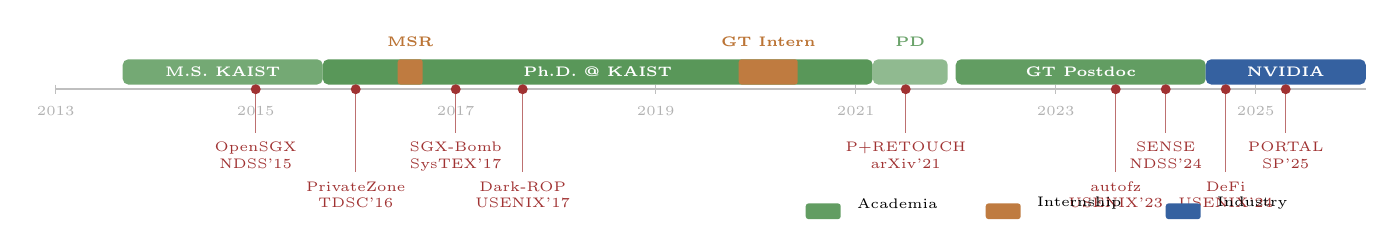
\begin{tikzpicture}[x=1.27cm, y=1.0cm, font=\scriptsize]

  % ---- axis line ----
  \draw[gray!50, line width=0.6pt] (0,0) -- (13.1,0);

  % ---- tick marks + year labels ----
  \foreach \yr/\lbl in {0/2013,2/2015,4/2017,6/2019,8/2021,10/2023,12/2025}{
    \draw[gray!50] (\yr, 0.06) -- (\yr, -0.06);
    \node[gray!60, anchor=north, font=\tiny] at (\yr, -0.1) {\lbl};
  }

  % ---- role bars (height 0.32, centred on y=0.22) ----
  % bar macro: \roleBar{xstart}{xend}{color}{label}
  % M.S. @ KAIST  Sep2013--Aug2015  -> 0.67..2.67
  \fill[rounded corners=2pt, cAcademia!75]
    (0.67, 0.06) rectangle node[font=\tiny\bfseries, white] {M.S.\ KAIST} (2.67, 0.38);
  % Ph.D. @ KAIST  Aug2015--Feb2021 -> 2.67..8.17
  \fill[rounded corners=2pt, cAcademia!90]
    (2.67, 0.06) rectangle node[font=\tiny\bfseries, white] {Ph.D.\ @ KAIST} (8.17, 0.38);
  % MSR Intern  May--Aug 2016 -> 3.42..3.67
  \fill[rounded corners=1pt, cIntern!85]
    (3.42, 0.06) rectangle (3.67, 0.38);
  \node[cIntern!90, anchor=south, font=\tiny\bfseries] at (3.545, 0.42) {MSR};
  % GT Intern  Nov2019--May2020 -> 6.83..7.42
  \fill[rounded corners=1pt, cIntern!85]
    (6.83, 0.06) rectangle (7.42, 0.38);
  \node[cIntern!90, anchor=south, font=\tiny\bfseries] at (7.125, 0.42) {GT Intern};
  % KAIST Postdoc  Mar--Dec 2021 -> 8.17..8.92
  \fill[rounded corners=2pt, cAcademia!60]
    (8.17, 0.06) rectangle (8.92, 0.38);
  \node[cAcademia!80, anchor=south, font=\tiny\bfseries] at (8.545, 0.42) {PD};
  % GT Postdoc  Jan2022--Jul2024 -> 9.0..11.5
  \fill[rounded corners=2pt, cAcademia!85]
    (9.0, 0.06) rectangle node[font=\tiny\bfseries, white] {GT Postdoc} (11.5, 0.38);
  % NVIDIA  Jul2024--present -> 11.5..13.1
  \fill[rounded corners=2pt, cIndustry!90]
    (11.5, 0.06) rectangle node[font=\tiny\bfseries, white] {NVIDIA} (13.1, 0.38);

  % ---- publication pins (stem down from axis, label below) ----
  % Each pin: dot on axis, stem, short label
  % Alternating depths -0.55 / -0.95 to avoid overlap
  % pin macro (inline): dot at (x,0), stem to (x, depth), label below
  \def\pina{-0.55}  % shallow
  \def\pinb{-1.05}  % deep

  % OpenSGX NDSS'15  x=2.0  -> shallow
  \draw[cPaper!70, line width=0.5pt] (2.0,0) -- (2.0,\pina);
  \fill[cPaper] (2.0,0) circle (1.8pt);
  \node[cPaper, anchor=north, align=center, font=\tiny] at (2.0,\pina) {OpenSGX\\NDSS'15};

  % PrivateZone TDSC'16  x=3.0  -> deep
  \draw[cPaper!70, line width=0.5pt] (3.0,0) -- (3.0,\pinb);
  \fill[cPaper] (3.0,0) circle (1.8pt);
  \node[cPaper, anchor=north, align=center, font=\tiny] at (3.0,\pinb) {PrivateZone\\TDSC'16};

  % SGX-Bomb SysTEX'17  x=4.0  -> shallow
  \draw[cPaper!70, line width=0.5pt] (4.0,0) -- (4.0,\pina);
  \fill[cPaper] (4.0,0) circle (1.8pt);
  \node[cPaper, anchor=north, align=center, font=\tiny] at (4.0,\pina) {SGX-Bomb\\SysTEX'17};

  % Dark-ROP USENIX'17  x=4.67  -> deep
  \draw[cPaper!70, line width=0.5pt] (4.67,0) -- (4.67,\pinb);
  \fill[cPaper] (4.67,0) circle (1.8pt);
  \node[cPaper, anchor=north, align=center, font=\tiny] at (4.67,\pinb) {Dark-ROP\\USENIX'17};

  % P+RETOUCH arXiv'21  x=8.5  -> shallow
  \draw[cPaper!70, line width=0.5pt] (8.5,0) -- (8.5,\pina);
  \fill[cPaper] (8.5,0) circle (1.8pt);
  \node[cPaper, anchor=north, align=center, font=\tiny] at (8.5,\pina) {P+RETOUCH\\arXiv'21};

  % autofz USENIX'23  x=10.6  -> deep
  \draw[cPaper!70, line width=0.5pt] (10.6,0) -- (10.6,\pinb);
  \fill[cPaper] (10.6,0) circle (1.8pt);
  \node[cPaper, anchor=north, align=center, font=\tiny] at (10.6,\pinb) {autofz\\USENIX'23};

  % SENSE NDSS'24  x=11.1  -> shallow
  \draw[cPaper!70, line width=0.5pt] (11.1,0) -- (11.1,\pina);
  \fill[cPaper] (11.1,0) circle (1.8pt);
  \node[cPaper, anchor=north, align=center, font=\tiny] at (11.1,\pina) {SENSE\\NDSS'24};

  % DeFi USENIX'24  x=11.7  -> deep
  \draw[cPaper!70, line width=0.5pt] (11.7,0) -- (11.7,\pinb);
  \fill[cPaper] (11.7,0) circle (1.8pt);
  \node[cPaper, anchor=north, align=center, font=\tiny] at (11.7,\pinb) {DeFi\\USENIX'24};

  % PORTAL SP'25  x=12.3  -> shallow
  \draw[cPaper!70, line width=0.5pt] (12.3,0) -- (12.3,\pina);
  \fill[cPaper] (12.3,0) circle (1.8pt);
  \node[cPaper, anchor=north, align=center, font=\tiny] at (12.3,\pina) {PORTAL\\SP'25};

  % ---- legend (bottom right) ----
  \fill[rounded corners=1pt, cAcademia!85] (7.5,-1.65) rectangle (7.85,-1.45)
    node[right, black, font=\tiny] {\ Academia};
  \fill[rounded corners=1pt, cIntern!85]   (9.3,-1.65) rectangle (9.65,-1.45)
    node[right, black, font=\tiny] {\ Internship};
  \fill[rounded corners=1pt, cIndustry!90] (11.1,-1.65) rectangle (11.45,-1.45)
    node[right, black, font=\tiny] {\ Industry};

\end{tikzpicture}%
}% end resizebox
}
\end{comment}


\begin{document}

\begin{center}
    {\huge \scshape JAEHYUK LEE, Ph.D.} \\ \vspace{1pt}
    \small
    \raisebox{-0.1\height}\faPhone\ 470-861-6020 ~
    \href{https://ruach.github.io}{\faHome\ https://ruach.github.io} ~
    \href{mailto:jaehyukl@nvidia.com}{\faEnvelope\ jaehyukl@nvidia.com} ~
   % \href{https://www.linkedin.com/in/jaehyuk-lee-29b33b121/}{\faLinkedin\ Jaehyuk Lee}  ~
    \vspace{-10pt}
\end{center}
%
%% ---- Career Timeline ----
%\vspace{2pt}
%\noindent\timelineChart
%\vspace{4pt}
%%
\section{SUMMARY}
\begin{interestbox}
\small\emph{I work on high-assurance systems security: Trusted Execution Environments, cryptographic attestation and root-of-trust, and hypervisor/OS isolation, paired with the adversarial side (side-channel attacks, exploit development, and fuzzing) to test whether those guarantees hold. Throughout my career, I have tackled security problems across the full hardware-software stack, driven by a desire to turn complex research problems into production-ready solutions.}
\end{interestbox}
\vspace{-3pt}
%
\section{WORK EXPERIENCE}
\vspace{1pt}
  \resumeSubHeadingListStart
    \resumeSubheading
      {Senior Security Engineer: NVIDIA Corporation, Santa Clara, CA}{Jul 2024 -- Current}
      {Title}{Location}
\resumeItemListStart

\resumeItem{Owned an end-to-end cryptographic attestation chain from silicon root of trust to signed evidence for Vera and Grace CC.}
\resumeItemListStart
    \resumeItem{Developed cross-layer firmware and software stacks across bootloader, RMM, ATF, PSCFW, and Caliptra DPE to enable end-to-end attestation and evidence generation for Vera CCA and Baremetal Secure AI on Vera and Grace CPUs.}
    \resumeItem{Developed and deployed CoRIM/CoMID manifests for Vera CCA and Vera/Grace baremetal attestation.}
\resumeItemListEnd
%
\vspace{4pt}
\resumeItem{Led Live Firmware Activation (LFA) support for RMM, building the software stack across RMM, ATF, and Vera IROT.}
%
\resumeItem{Hardened guest OS boot sequence and model loading using initramfs disk encryption with early attested key provisioning.}
    \resumeItemListEnd
    \resumeSubheading
      {Postdoc Researcher: Georgia Institute of Technology, Atlanta, GA}{Jan 2022 -- Jul 2024}
      {Title}{Location}
      \resumeItemListStart
        \resumeItem {Developed an automated fuzzer selection tool that dynamically selected fuzzers based on runtime analysis \ref{paper:autofz}} %Anyone having no knowledge of fuzzers can simply utilize it for automate vulnerability discovery}
        \resumeItem {Designed and implemented a hardware-enforced secure I/O path between confidential VMs and DMA peripherals ~\ref{paper:portal}}
        %(GPUs) by moving IOMMU (SMMU) page-table ownership into the TEE's trust boundary under ARM CCA, replacing per-transfer encryption with isolation guarantees~\ref{paper:portal}} %\resumeItem {Developed expertise in managing 30+ node multi-rack server environments and diagnosing end-to-end hardware and software issues}
        \resumeItem {Conducted vulnerability research on Intel and ARM's latest hardware-isolated confidential VM architectures (TDX \& CCA)}
    \resumeItemListEnd
     
    \resumeSubheading
      {Postdoc Researcher: \small{Korea Advanced Institute of Science and Technology}, Korea}{Mar 2021 -- Dec 2021}
      {Title}{Location}
      \resumeItemListStart
        \resumeItem {Demonstrated an eviction-free cache side-channel attack on x86 and Apple M1, bypassing eviction-monitoring defenses~\ref{paper:cache-attack}}
        \resumeItem{Assisted in supervising and mentoring Ph.D. students across a large research group (20+ members).}


    \resumeItemListEnd
   
    \resumeSubheading
      {Research Intern: Georgia Institute of Technology, Atlanta, GA}{Nov 2019 -- May 2020}
      {Title}{Location}
      \resumeItemListStart
        \resumeItem{Developed a hardware-based side-channel mitigation system on GEM5, monitoring cache and TLB eviction events~\ref{paper:sense}}
        %(cache and TLB evictions) \ref{paper:sense}}
    \resumeItemListEnd

    \resumeSubheading
      {Research Intern: Microsoft Research, Redmond, WA}{May 2016 -- Aug 2016}
      {Title}{Location}
      \resumeItemListStart
        \resumeItem{Executed practical ROP attacks on Intel SGX by exploiting memory corruption vulnerabilities without binary details~\ref{paper:sgx-rop}}
        %
        \resumeItem{Developed a secure CDN enabling enterprises to offload sensitive user data to untrusted third-party cloud providers.}
    \resumeItemListEnd
  \resumeSubHeadingListEnd
%------------Publications-----------

\section{PUBLICATION \& PATENT \small\href{https://scholar.google.com/citations?user=nfpCTgUAAAAJ&hl=en}{(829 citations)}}
\emph{Top-tier conferences (\textcolor{venuecolor}{SP, USENIX Security, NDSS}) and Journal (\textcolor{venuecolor}{TDSC})}
\vspace{2pt}
    \resumeSubHeadingListLabelStart
%
    \resumeProjectHeadingWithLabel
    {\textbf{PORTAL: Fast and Secure Device Access with Arm CCA for Modern Arm Mobile SoC} $|$
    \href{https://www.computer.org/csdl/proceedings-article/sp/2025/223600a013/21B7Q5c3ZHq}{Paper}}
    {SP 2025}{paper:portal}
    \resumeItemListStart
        \resumeItem{Eliminated per-transfer encryption overhead for Arm CCA Realm VMs accessing DMA-capable peripherals.}
        %by migrating SMMU stage-2 page table ownership into TF-RMM and introducing new RMI calls (\texttt{RMI\_DEVICE\_ATTACH/DETACH}) between KVM and RMM, enabling hardware-enforced isolated DMA regions without cryptographic cost.}
        \resumeItem{Extended the Linux SMMU driver to delegate page table management to RMM; implemented the Realm-side driver and the full RMI call path across KVM, TF-RMM, and the SMMU hardware controller. Modified the RMM implementation to enable hardware-enforced (GPT) isolated DMA regions without cryptographic operation.}
    \resumeItemListEnd
%
    %
    \resumeProjectHeadingWithLabel
    {\textbf{SENSE: Enhancing Microarchitectural Awareness via Subscription-Based Notification}
    $|$
    \href{https://www.ndss-symposium.org/wp-content/uploads/2024-176-paper.pdf}{Paper}
    }{NDSS 2024}{paper:sense}
%
    \resumeItemListStart
        \resumeItem{Addressed the lack of microarchitectural visibility in TEEs, which left them blind to cache/TLB side-channel attacks.}
        %by designing a subscription-based ISA extension that delivers hardware events directly to the enclave handler --- without requiring OS cooperation.}
        \resumeItem{Extended the GEM5 out-of-order CPU pipeline with new micro-ops and added event-tracking metadata bits to the cache and TLB models; implemented the enclave-side handler dispatch path.}
    \resumeItemListEnd
%
    \resumeProjectHeadingWithLabel
    {\textbf{autofz: Automated Fuzzer Composition at Runtime} $|$
    \href{https://www.usenix.org/system/files/sec23fall-prepub-446-fu.pdf}{Paper}
    $|$
    \href{https://news.ycombinator.com/item?id=34977319}{Hacker News}}{USENIX 2023}{paper:autofz}
    \resumeItemListStart
        \resumeItem{Eliminated the need for per-target fuzzer selection by building a runtime coordinator that measures each fuzzer's coverage.}
        %via AFL bitmaps and reallocates CPU time with AIMD, lifting bug-finding throughput by up to 3$\times$ over the best single fuzzer across 12 targets.}
        \resumeItem{Implemented the orchestration layer in Python using Linux cgroups for CPU pinning; integrated 12 fuzzers (AFL, AFLFast, MOpt, RedQueen, QSYM, Angora, and others) under a unified coverage-feedback interface.}
    \resumeItemListEnd
%
    \resumeProjectHeadingWithLabel
    {\textbf{Hacking in Darkness: Return-oriented Programming against Secure Enclaves}
    $|$ \href{https://www.usenix.org/system/files/conference/usenixsecurity17/sec17-lee-jaehyuk.pdf}{Paper} $|$
    \href{https://www.youtube.com/watch?v=NP7f3M_saUs}{Talk} $|$
    \href{https://www.youtube.com/watch?v=hyuZFf3QxvM}{Demo}
    }{USENIX 2017}{paper:sgx-rop}
    \resumeItemListStart
        \resumeItem{Demonstrated the first ROP attack against Intel SGX: exploited the deterministic AEX fault oracle to probe enclave memory word-by-word and reconstruct a gadget map \emph{without any binary knowledge} and showcased full key exfiltration.}
        \resumeItem{Built the AEX-based memory scanner and ROP-chain generator in C/x86 assembly; reverse-engineered Intel SGX library (e.g., EPCM/TCS/SSA layouts) to locate gadgets and craft the exploit entirely from outside the enclave.}
    \resumeItemListEnd
%
    \resumeProjectHeadingWithLabel
    {\textbf{SGX-Bomb: Locking Down the Processor via Rowhammer Attack} $|$
    \href{https://www.unexploitable.systems/uploads/jang:sgx-bomb.pdf}{Paper} $|$
    \href{https://news.ycombinator.com/item?id=15743608}{Hacker News} $|$
    \href{https://www.youtube.com/watch?v=HUAyTLV_Mao}
    {Demo}
    }{SysTEX 2017}{paper:sgx-bomb}
    \resumeItemListStart
        \resumeItem{Showed that an enclave can weaponize Rowhammer to permanently lock the Memory Encryption Engine (MEE) and force a machine reboot --- rendering SGX's integrity guarantees a denial-of-service vector for cloud multi-tenant scenarios.}
        \resumeItem{Wrote a kernel driver to reverse-engineer DRAM bank/row mapping from physical addresses; implemented the double-sided Rowhammer loop in x86 assembly inside an enclave to flip MEE metadata bits and trigger a machine lockdown.}
    \resumeItemListEnd
%
    \resumeProjectHeadingWithLabel
    {\textbf{PrivateZone: Providing a Private Execution Environment using ARM TrustZone} $|$ \href{https://cysec.kr/publications/PrivateZone_Providing_a_Private_Execution_Environment_using_ARM_TrustZone.pdf}{Paper}
    }{TDSC 2016}{paper:privateZone}
    \resumeItemListStart
        \resumeItem{Extended ARM TrustZone to protect arbitrary user-space processes without porting them to the Secure World, by intercepting Linux scheduling events in Monitor mode and switching per-process stage-2 page tables on each context switch.}
        \resumeItem{Implemented the stage-2 page table allocator and the Monitor-mode context-switch handler in ARM assembly; modified the Linux scheduler to emit SVC calls that trigger the switch between trusted and untrusted page tables.}
       
    \resumeItemListEnd

%
    \resumeProjectHeadingWithLabel
    {\textbf{OpenSGX: An Open Platform for SGX Research} $|$ \href{https://taesoo.kim/pubs/2016/jain:opensgx.pdf}{Paper} $|$
    \href{https://en.wikipedia.org/wiki/Software_Guard_Extensions}{Wikipedia: SGX}}{NDSS 2015}{paper:open-sgx}
    \resumeItemListStart
        \resumeItem{Lowered the barrier to SGX research by building a QEMU instruction-level emulator that faithfully reproduced EPCM, SECS, TCS, and SSA data structures, enabling enclave development without SGX-enabled hardware.}
        \resumeItem{Implemented \texttt{EENTER}/\texttt{EEXIT} context-switch stubs in x86 assembly, EPCM management in QEMU's softmmu, and a \texttt{sgxlib} user library with a stub-call layer that routes enclave system calls through an untrusted trampoline.}
    \resumeItemListEnd
%  
    \resumeProjectHeadingWithLabel
    {\textbf{PRIME+RETOUCH: When Cache is Locked and Leaked} $|$
    \href{https://arxiv.org/abs/2402.15425}{Paper}}{arXiv}{paper:cache-attack}
    \resumeItemListStart
        \resumeItem{Identified a blind spot in eviction-based defenses: Tree-PLRU metadata can be manipulated to ``retouch'' a cache set so the victim line survives eviction silently, bypassing Intel TSX-based monitors and Apple M1 PMU counters.}
        \resumeItem{Reverse-engineered the Tree-PLRU state machine on recent Intel and Apple M1 caches; built the PRIME+RETOUCH PoC in x86/ARM assembly using pointer-chasing and memory barriers; demonstrated cross-core and cross-process secret recovery.}
    \resumeItemListEnd
%
     \resumeProjectHeadingWithLabel
    {\textbf{Survey On DeFi Users’ Perception of Security Breaches and Countermeasures} $|$
    \href{https://www.usenix.org/conference/usenixsecurity24/presentation/liu-mingyi}{Paper}}
    {USENIX 2024}{paper:defi}
        \resumeItemListStart
        \resumeItem{Revealed that DeFi victims overwhelmingly skip post-incident security review and instead seek new platforms to recover losses quickly, suggesting industry regulation is more effective than user education alone.}
        \resumeItem{Conducted semi-structured interviews and surveys; performed qualitative coding of transcripts using Dedoose.}
    \resumeItemListEnd
%
   \resumeProjectHeadingWithLabel
    {\textbf{A Rule Extraction Method Using Relevance Factor for FMM Neural Networks} $|$
    \href{https://koreascience.kr/article/JAKO201319947249078.page}{Paper}
    }{KTSDE 2013}{paper:FMM}
    \resumeItemListStart
        \resumeItem{
        Enhanced the Fuzzy Min-Max (FMM) neural network by incorporating the frequency of features in training.}
        \resumeItem{
        Reduced classification ambiguity by weighting feature relevance and frequency during training.}
    \resumeItemListEnd
%
    \resumeProjectHeadingWithLabel
    {\textbf{Apparatus and method for open and private IoT gateway using Intel SGX} $|$ \href{https://patents.google.com/patent/KR102162018B1/en}{Patent}}{KR102162018B1}{patent:iot-gateway}
    \resumeItemListStart
        \resumeItem{
Designed a secure IoT gateway utilizing Intel SGX for protocol conversion, encrypted data transfer, and enclave-based key management across cross-platform communication channels.}
    \resumeItemListEnd
    \resumeSubHeadingListLabelEnd

% adjust vscape based on the space you want to leave between each section.
\section{SOFTWARE ARTIFACTS}
\resumeSubHeadingListStart
    \softwareArtifactHeading
    {\makebox[2.2cm][l]{\textbf{Autofz:}} {\href{https://github.com/sslab-gatech/autofz}{\faGithub  \hspace{0.1em} https://github.com/sslab-gatech/autofz}}}
    {\makebox[1.0cm][l]{\faCodeFork 12} \makebox[1.0cm][l]{\faStar 85}}
    %
    \softwareArtifactHeading
    {\makebox[2.2cm][l]{\textbf{OpenSGX:}} {\href{https://github.com/sslab-gatech/opensgx}{\faGithub  \hspace{0.1em} https://github.com/sslab-gatech/opensgx}}}
    {\makebox[1.0cm][l]{\faCodeFork 82} \makebox[1.0cm][l]{\faStar 308}}
    %
     \softwareArtifactHeading
    {\makebox[2.2cm][l]{\textbf{SGXBomb:}} {\href{https://github.com/sslab-gatech/sgx-bomb}{\faGithub  \hspace{0.1em} https://github.com/sslab-gatech/sgx-bomb}}}
    {\makebox[1.0cm][l]{\faCodeFork 4} \makebox[1.0cm][l]{\faStar 18}}
\resumeSubHeadingListEnd
\vspace{7pt}

\begin{comment}
%-----------PROJECTS-----------
\section{SELECTED PROJECTS}
    \resumeSubHeadingListStart
    \resumeProjectHeadingNoBold
          {\textbf{Enabling Rack-scale Disaggregation-aware Confidential Computing via Intel IPUs}}
          {{Intel Lab (On-going)}}
          \resumeItemListStart
            \resumeItem{Modern data centers disaggregate hardware for efficiency, but TEE lacks seamless communication with disaggregated resources. This project seeks to enhance TEE using Intel IPUs to establish secure channels within and across racks.}
          \resumeItemListEnd
%
    \resumeProjectHeadingNoBold
          {\textbf{Exploring Possible Vulnerabilities in Intel TDX}}
          {{Intel Lab (On-going)}}
          \resumeItemListStart
            \resumeItem{TEEs for confidential VMs, create a unique threat model where trust cannot be placed in the host VMM and OS while still being essential for resource management. We investigate potential side channels due to this new threat model.}
          \resumeItemListEnd
%
    \resumeProjectHeadingNoBold
          {\textbf{Research for Virtual Machine Introspection (VMI) for Linux KVM }}
          {{Nation Security Research Institute}}
          \resumeItemListStart
            \resumeItem{Developed a VMI library for Linux KVM enabling inspection of VM status, including memory and registers. Modified EPT management code and its fault handler to monitor malicious memory access events.}
            \resumeItem{
            Created an interface between QEMU and the KVM kernel module to enable the registration of events for monitoring suspicious memory access and updates.}
        \resumeItemListEnd
%
    \resumeProjectHeadingNoBold
    {\textbf{OS Kernel Behavior Modeling for Introspection}}
    {{Agency for Defense Development}}
    \resumeItemListStart
        \resumeItem{
        Extracted invariants to capture the benign behavior of the Linux kernel, utilizing the Daikon dynamic invariant detection tool.}
        \resumeItem{
        Deployed Control Flow Integrity (CFI) for the Linux kernel, leveraging extracted invariants as the guiding principle to detect anomalous behavior.}
    \resumeItemListEnd
%%
    \resumeProjectHeadingNoBold
    {\textbf{Introspection Platform for Trusted Execution Environment (TEE)}}
    {{National Security Research Institute (NSRI)}}
    \resumeItemListStart
        \resumeItem{
      Developed compiler-based monitoring software operating within Intel SGX, aimed at tracing all ENCLU instructions invoked within SGX enclaves to record security-critical events.}
       
    \resumeItemListEnd
    \resumeSubHeadingListEnd
\end{comment}
%
\section{TECHNICAL SKILLS}
\begin{itemize}[leftmargin=0.1in, label={}, itemsep=1pt, topsep=0pt, parsep=0pt]
    \item \small\textbf{Software}: C, C++, Rust, Scala, Python, TF-A, TF-RMM, Caliptra FW, PSC FW (NVIDIA IROT), Linux Kernel, KVM, QEMU, ARM/X86 Assembly, Fuzzing, GDB, CoCLI
    \item \small\textbf{Hardware}: GEM5 (x86 simulator), Processor Pipeline, Cache, TLB, Microcode, HW Side Channel, (System)Verilog, Chisel (RISC-V), Intel SGX \& TDX, ARM CCA \& TrustZone, IOMMU, PCIe
    \item \small\textbf{Spec}: Entity Attestation Token (EAT), Concise Reference Integrity Manifest (CoRIM), DICE Protection Environment (DPE), Security Protocol and Data Model (SPDM), TEE Device Interface Security Protocol (TDISP)
\end{itemize}
\vspace{-3pt}
%
\section{EDUCATION}
\begin{tabular*}{\textwidth}{@{\extracolsep{\fill}}lllp{3.5cm}r@{}}
    \textbf{Institution} & \textbf{Degree} & \textbf{Field of Study} & \textbf{Dates} & \textbf{GPA} \\
    Korea Advanced Institute of Science and Technology & \emph{Ph.D.} & Information Security & Aug 2015 -- Feb 2021 & {3.95} \\
    {Korea Advanced Institute of Science and Technology} & \emph{M.S.} & Information Security & Sep 2013 -- Aug 2015 & {4.1} \\
    {Handong Global University} & \emph{B.S.} & Computer Science & Mar 2010 -- Aug 2013 & {4.2}
\end{tabular*}
\vspace{-6pt}
%
\section{PROFESSIONAL ACTIVITIES}

    \resumeSubHeadingListLabelStart
    \item {\textbf{Journal Review}}
    \begin{itemize}[leftmargin=*, itemsep=4pt, topsep=1pt, parsep=0pt, partopsep=0pt]
        \item\small\begin{tabular*}{0.97\textwidth}{l@{\extracolsep{\fill}}r}
            IEEE Transactions on Dependable and Secure Computing & {\href{https://ieeexplore.ieee.org/xpl/RecentIssue.jsp?punumber=8858}{Impact Factor: 7.3}},\ \emph{2024}
        \end{tabular*}\vspace{-4pt}
        \item\small\begin{tabular*}{0.97\textwidth}{l@{\extracolsep{\fill}}r}
            Computer \& Security & {\href{https://shop.elsevier.com/journals/computers-and-security/0167-4048}{Impact Factor: 5.7}},\ \emph{2024}
        \end{tabular*}\vspace{-4pt}
        \item\small\begin{tabular*}{0.97\textwidth}{l@{\extracolsep{\fill}}r}
            Journal of Information Security and Applications & {\href{https://www.sciencedirect.com/journal/journal-of-information-security-and-applications}{Impact Factor: 5.6}},\ \emph{2024}
        \end{tabular*}\vspace{-4pt}
        \item\small\begin{tabular*}{0.97\textwidth}{l@{\extracolsep{\fill}}r}
            IEEE Access & {\href{https://ieeeaccess.ieee.org/about-ieee-access/learn-more-about-ieee-access/}{Impact Factor: 3.9}},\ \emph{2024}
        \end{tabular*}\vspace{-4pt}
        \item\small\begin{tabular*}{0.97\textwidth}{l@{\extracolsep{\fill}}r}
            ACM Transactions on Internet Technology & {\href{https://dl.acm.org/journal/toit/indexing}{Impact Factor: 3.9}},\ \emph{2024}
        \end{tabular*}\vspace{-4pt}
        \item\small\begin{tabular*}{0.97\textwidth}{l@{\extracolsep{\fill}}r}
            IEEE Journal of Communications and Networks & {\href{https://ieeexplore.ieee.org/xpl/RecentIssue.jsp?punumber=5449605}{Impact Factor: 3.6}},\ \emph{2024}
        \end{tabular*}\vspace{-4pt}
    \end{itemize}
%
    \item {\textbf{Conference Review}}
    \begin{itemize}[leftmargin=*, itemsep=4pt, topsep=1pt, parsep=0pt, partopsep=0pt]
        \item\small\begin{tabular*}{0.97\textwidth}{l@{\extracolsep{\fill}}r}
            IEEE Mobile Ad Hoc and Smart Systems (MASS) & \emph{2024}
        \end{tabular*}\vspace{-4pt}
        \item\small\begin{tabular*}{0.97\textwidth}{l@{\extracolsep{\fill}}r}
            IEEE International Conference on Parallel and Distributed Systems (ICPADS) & \emph{2024}
        \end{tabular*}\vspace{-4pt}
    \end{itemize}

    \item {\textbf{External Reviewer}}
    \begin{itemize}[leftmargin=*, itemsep=4pt, topsep=1pt, parsep=0pt, partopsep=0pt]
        \item\small\begin{tabular*}{0.97\textwidth}{l@{\extracolsep{\fill}}r}
            IEEE Symposium on Security and Privacy (Oakland) & \emph{2016, 2017, 2018, 2020, 2021, 2022}
        \end{tabular*}\vspace{-4pt}
        \item\small\begin{tabular*}{0.97\textwidth}{l@{\extracolsep{\fill}}r}
            USENIX Security Symposium (Security) & \emph{2015, 2021, 2022, 2023, 2024}
        \end{tabular*}\vspace{-4pt}
        \item\small\begin{tabular*}{0.97\textwidth}{l@{\extracolsep{\fill}}r}
            ACM Conference on Computer and Communications Security (CCS) & \emph{2015, 2017, 2018, 2019, 2023}
        \end{tabular*}\vspace{-4pt}
        \item\small\begin{tabular*}{0.97\textwidth}{l@{\extracolsep{\fill}}r}
            Network and Distributed System Security Symposium (NDSS) & \emph{2019, 2020, 2021}
        \end{tabular*}\vspace{-4pt}
        \item\small\begin{tabular*}{0.97\textwidth}{l@{\extracolsep{\fill}}r}
            ACM ASIA Conference on Computer and Communications Security (ASIACCS) & \emph{2015, 2016, 2018}
        \end{tabular*}\vspace{-4pt}
        \item\small\begin{tabular*}{0.97\textwidth}{l@{\extracolsep{\fill}}r}
            ACM Symposium on Operating Systems Principles (SOSP) & \emph{2021}
        \end{tabular*}\vspace{-4pt}
        \item\small\begin{tabular*}{0.97\textwidth}{l@{\extracolsep{\fill}}r}
            ACM International World Wide Web Conference (WWW) & \emph{2018}
        \end{tabular*}\vspace{-4pt}
    \end{itemize}
    \resumeSubHeadingListLabelEnd
   

\section {INVITED TALKS}
    \resumeSubHeadingListLabelStart
    \item {\small\textbf{A Novel Cache Side Channel Attack without Attacker Eviction}}
    \resumeItemListStart
        \resumeItem{Presented at Intel Side Channel Academic Program (SCAP), Virtual, Sep 2020}
    \resumeItemListEnd
    %
    \item {\small\textbf{Hacking in Darkness: Return-oriented Programming against Secure Enclaves}}
    \resumeItemListStart
        \resumeItem{Presented at the 26th USENIX Security $|$ \href{https://www.youtube.com/watch?v=NP7f3M_saUs}{Presentation Link}, Vancouver, BC, Canada, Aug 2017}
        \resumeItem{Presented at KimchiCon $|$ \href{https://www.youtube.com/watch?v=gC4vZ7BjZxA}{Presentation Link}, Daejeon, South Korea, Aug 2017}
    \resumeItemListEnd
    %
    \item {\small\textbf{Tutorial: Trusted Execution Environment: TrustZone, ITP and SGX}}
    \resumeItemListStart
        \resumeItem{Korea Institute of Information Security and Cryptology, Seoul, South Korea, Apr 2015}
    \resumeItemListEnd
    \resumeSubHeadingListLabelEnd
\vspace{7pt}

\section {THESIS}
    \resumeSubHeadingListStart
    \item
    \begin{tabular*}{1.00\textwidth}{l@{\extracolsep{\fill}}r}
      \parbox{0.8\textwidth}{\emph{\small Unintended Consequences of System Design: Unpremeditated Usage of Benign System Components Devastates Security}} & {\small Ph.D. Thesis.} \\
    \end{tabular*}\vspace{-3pt}
    %
    \resumeProjectHeadingNoBold
          {\emph{Detecting Emulated Environment: Exploiting Behavioral Discrepancies in QEMU}}
          {{M.S. Thesis.}}
    \resumeSubHeadingListEnd

\begin{comment} % Research Impact Summary — move here to re-enable
% ---- Research Impact Summary ----
\vspace{2pt}
{\small
\renewcommand{\arraystretch}{1.15}
\noindent\begin{tabular*}{\textwidth}{@{}l@{\hspace{6pt}}l@{\hspace{10pt}}r@{\hspace{8pt}}l@{\hspace{6pt}}l@{}}
\toprule
\textbf{Paper} & \textbf{Venue} & \textbf{Cite} & \textbf{Impact} & \textbf{System Layer} \\
\midrule
Dark-ROP          & USENIX Sec.'17 & 274 & \textcolor{gray!80}{\rule{60pt}{4pt}} & Kernel, HW \\
SGX-Bomb          & SysTEX'17      & 265 & \textcolor{gray!80}{\rule{58pt}{4pt}} & Hardware (DRAM) \\
OpenSGX           & NDSS'15        & 144 & \textcolor{gray!80}{\rule{32pt}{4pt}} & HW $\to$ Kernel $\to$ User \\
PrivateZone       & TDSC'16        &  84 & \textcolor{gray!80}{\rule{18pt}{4pt}} & Firmware, Kernel \\
PORTAL            & SP'25          &  21 & \textcolor{gray!80}{\rule{5pt}{4pt}}  & Firmware, Kernel, Driver \\
autofz            & USENIX Sec.'23 &  22 & \textcolor{gray!80}{\rule{5pt}{4pt}}  & User-space \\
DeFi Survey       & USENIX Sec.'24 &  15 & \textcolor{gray!80}{\rule{3pt}{4pt}}  & --- \\
P+RETOUCH         & arXiv'24       &   1 & \textcolor{gray!80}{\rule{1pt}{4pt}}  & Hardware (Cache) \\
SENSE             & NDSS'24        &   2 & \textcolor{gray!80}{\rule{1pt}{4pt}}  & HW Sim (GEM5) \\
\bottomrule
\multicolumn{5}{@{}l@{}}{\tiny Citations: Google Scholar, Jul 2026. Bar $\propto$ citation count (max 274).}
\end{tabular*}
}
\vspace{2pt}
\end{comment}
\end{document}
